% arara: indent: { overwrite: yes }
% arara: latexmk: { engine: xelatex }
\documentclass[
	% -- opções da classe memoir --
	12pt,				% tamanho da fonte
	openright,			% capítulos começam em pág ímpar (insere página vazia caso preciso)
	twoside,			% para impressão em recto e verso. Oposto a oneside
	a4paper,			% tamanho do papel. 
	% -- opções do pacote babel --
%	english,			% idioma adicional para hifenização
%	brazil				% o último idioma é o principal do documento
	]{abntex2}

% ---
% Pacotes básicos 
% ---
\usepackage{lmodern}			% Usa a fonte Latin Modern			
\usepackage[T1]{fontenc}		% Selecao de codigos de fonte.
\usepackage{polyglossia}
\setdefaultlanguage[variant=brazilian]{portuguese}
%\usepackage[utf8]{inputenc}		% Codificacao do documento (conversão automática dos acentos)
\usepackage{indentfirst}		% Indenta o primeiro parágrafo de cada seção.
\usepackage{color}				% Controle das cores
\usepackage{graphicx}			% Inclusão de gráficos
\usepackage{microtype} 			% para melhorias de justificação


\usepackage{IMTtikz}
\DeclareSIUnit{\molar}{M}
\usepackage[version=4]{mhchem}

% ---
		
% ---
% Pacotes adicionais, usados apenas no âmbito do Modelo Canônico do abnteX2
% ---
%\usepackage{float}
\usepackage{wrapfig}
\usepackage{enumitem,quoting}
\usepackage{texshade}
% ---

% ---
% Pacotes de citações
% ---
\usepackage[brazilian,hyperpageref]{backref}	 % Paginas com as citações na bibl
\usepackage[alf]{abntex2cite}	% Citações padrão ABNT
\usepackage[all]{hypcap}
% --- 
% CONFIGURAÇÕES DE PACOTES
% --- 

% ---
% Configurações do pacote backref
% Usado sem a opção hyperpageref de backref
\renewcommand{\backrefpagesname}{Citado na(s) página(s):~}
% Texto padrão antes do número das páginas
\renewcommand{\backref}{}
% Define os textos da citação
\renewcommand*{\backrefalt}[4]{
	\ifcase #1 %
		Nenhuma citação no texto.%
	\or
		Citado na página #2.%
	\else
		Citado #1 vezes nas páginas #2.%
	\fi}%
% ---

% ---
% Informações de dados para CAPA e FOLHA DE ROSTO
% ---
\titulo{Prova 1 - Proteínas RAG-1 e RAG-2}
\autor{Isabella Basso do Amaral - 11810773}
\local{São Paulo, Brasil}
\data{}
%\makeatletter
%\makeatother
\orientador{Alicia Kowaltowski \& Sayuri Miyamoto}
%\coorientador{}
\renewcommand{\imprimirorientadorRotulo}{Professoras:}
\instituicao{%
  Universidade de São Paulo -- USP
  \par
  Curso de Ciências Moleculares
  \par
  Disciplina de Biologia I (CCM0111)}
\tipotrabalho{Prova I}
% O preambulo deve conter o tipo do trabalho, o objetivo, 
% o nome da instituição e a área de concentração 
\preambulo{Uma breve introdução às proteínas RAG-1 e RAG-2 e um método de purificação das mesmas.}
% ---


% ---
% Configurações de aparência do PDF final

% alterando o aspecto da cor azul
\definecolor{blue}{RGB}{41,5,195}

% informações do PDF
\makeatletter
\hypersetup{
     	%pagebackref=true,
		pdftitle={\@title}, 
		pdfauthor={\@author},
    	pdfsubject={\imprimirpreambulo},
	    pdfcreator={Isabella B},
		pdfkeywords={bio}{biologia}{CCM0111}{proteína}{P1}{prova}{RAG}, 
		colorlinks=true,       		% false: boxed links; true: colored links
    	linkcolor=blue,          	% color of internal links
    	citecolor=blue,        		% color of links to bibliography
    	filecolor=magenta,      		% color of file links
		urlcolor=blue,
		bookmarksdepth=4
}
\makeatother
% --- 

% ---
% Posiciona figuras e tabelas no topo da página quando adicionadas sozinhas
% em um página em branco. Ver https://github.com/abntex/abntex2/issues/170
\makeatletter
\setlength{\@fptop}{5pt} % Set distance from top of page to first float
\makeatother
% ---

% ---
% Possibilita criação de Quadros e Lista de quadros.
% Ver https://github.com/abntex/abntex2/issues/176
%
\newcommand{\quadroname}{Quadro}
\newcommand{\listofquadrosname}{Lista de quadros}

\newfloat[chapter]{quadro}{loq}{\quadroname}
\newlistof{listofquadros}{loq}{\listofquadrosname}
\newlistentry{quadro}{loq}{0}

% configurações para atender às regras da ABNT
\setfloatadjustment{quadro}{\centering}
\counterwithout{quadro}{chapter}
\renewcommand{\cftquadroname}{\quadroname\space} 
\renewcommand*{\cftquadroaftersnum}{\hfill--\hfill}

\setfloatlocations{quadro}{hbtp} % Ver https://github.com/abntex/abntex2/issues/176
% ---

% --- 
% Espaçamentos entre linhas e parágrafos 
% --- 

% O tamanho do parágrafo é dado por:
\setlength{\parindent}{1.3cm}

% Controle do espaçamento entre um parágrafo e outro:
\setlength{\parskip}{0.2cm}  % tente também \onelineskip

% ---
% compila o indice
% ---
\makeindex
% ---

% ----
% Início do documento
% ----
\begin{document}

% Seleciona o idioma do documento (conforme pacotes do babel)
%\selectlanguage{english}
\selectlanguage{brazil}

% Retira espaço extra obsoleto entre as frases.
\frenchspacing

% ----------------------------------------------------------
% ELEMENTOS PRÉ-TEXTUAIS
% ----------------------------------------------------------
% \pretextual

% ---
% Capa
% ---
\imprimircapa
% ---

% ---
% Folha de rosto
% (o * indica que haverá a ficha bibliográfica)
% ---
\imprimirfolhaderosto*
% ---

% ---
% RESUMOS
% ---

% resumo em português
%\setlength{\absparsep}{18pt} % ajusta o espaçamento dos parágrafos do resumo
%\begin{resumo}
%	Segundo a \cite{RAGintro}, o resumo deve ressaltar o
%	objetivo, o método, os resultados e as conclusões do documento. A ordem e a extensão
%	destes itens dependem do tipo de resumo (informativo ou indicativo) e do
%	tratamento que cada item recebe no documento original. O resumo deve ser
%	precedido da referência do documento, com exceção do resumo inserido no
%	próprio documento. (\ldots) As palavras-chave devem figurar logo abaixo do
%	resumo, antecedidas da expressão Palavras-chave:, separadas entre si por
%	ponto e finalizadas também por ponto.
%
%	\textbf{Palavras-chave}: proteína. purificação. RAG. gene ativador de recombinação. imunologia. anticorpos. recombinação V(D)J. recombinação somática.
%\end{resumo}

% resumo em inglês
%\begin{resumo}[Abstract]
% \begin{otherlanguage*}{english}
%   This is the english abstract.
%
%   \vspace{\onelineskip}
% 
%   \noindent 
%   \textbf{Keywords}: latex. abntex. text editoration.
% \end{otherlanguage*}
%\end{resumo}

% ---
% inserir lista de ilustrações
% ---
\pdfbookmark[0]{\listfigurename}{lof}
\listoffigures*
\cleardoublepage
% ---

% ---
% inserir lista de quadros
% ---
%\pdfbookmark[0]{\listofquadrosname}{loq}
%\listofquadros*
%\cleardoublepage
% ---

% ---
% inserir lista de tabelas
% ---

%\pdfbookmark[0]{\listtablename}{lot}
%\listoftables*
%\cleardoublepage
% ---

% ---
% inserir lista de abreviaturas e siglas
% ---
\begin{siglas}
	\item[D] \textit{Diversity}
	\item[DNA] \textit{Deoxyribonucleic acid}
	\item[DMEM] \textit{Dulbecco's modified Eagle medium}
	\item[EDTA] \textit{Ethylenediaminetetraacetic acid}
	\item[FBS] \textit{Fetal Bovine Serum}
	\item[HEK] \textit{Human Embryonic Kidney}
	\item[J] \textit{Joining}
	\item[LSB] \textit{Laemmli Sample Buffer}
	\item[MBP] \textit{Maltose Binding Protein}
	\item[PBS] \textit{Phosphate buffered saline}
	\item[PCR] \textit{Polymerase chain reaction}
	\item[PMSF] \textit{Phenylmethylsulfonyl fluoride}
	\item[PEI] \textit{Polyethylenimine}
	\item[RAG] \textit{Recombination activating gene}
	\item[RNA] \textit{Ribonucleic acid}
	\item[RSB] \textit{Resuspension Buffer}
	\item[RSS] \textit{Recombination signal sequence}
	\item[SDS-PAGE] \textit{Sodium Dodecyl Sulphate --- Polyacrylamide Gel Electrophoresis}
	\item[V] \textit{Variable}
	\item[WB] \textit{Western Blot}
\end{siglas}
% ---

% ---
% inserir lista de símbolos
% ---
%\begin{simbolos}
%	\item[$ \Gamma $] Letra grega Gama
%	\item[$ \Lambda $] Lambda
%	\item[$ \zeta $] Letra grega minúscula zeta
%	\item[$ \in $] Pertence
%\end{simbolos}
% ---

% ---
% inserir o sumario
% ---
\pdfbookmark[0]{\contentsname}{toc}
\tableofcontents*
\cleardoublepage
% ---



% ----------------------------------------------------------
% ELEMENTOS TEXTUAIS
% ----------------------------------------------------------
\textual


\chapter{Introdução}

As RAGs (\textit{Recombination activating genes}) são proteínas responsáveis por parte do processo conhecido como \textbf{recombinação V(D)J} (explicado em \citeonline{introMain,introMain2}), onde V, D e J são siglas para os termos \textit{variable} (ou variável), \textit{diversity} (ou diversidade) e \textit{joining} (ou junção), respectivamente.

A recombinação V(D)J é um processo essencial para a imunidade humana, pois é ela a responsável pela diversidade no repertório de anticorpos, ocorrendo nas etapas iniciais de maturação de linfócitos B e T. Ela promove a formação de exons a partir dos segmentos gênicos V e J, podendo incluir um segmento D também.

%\begin{figure}
%	\centering
%	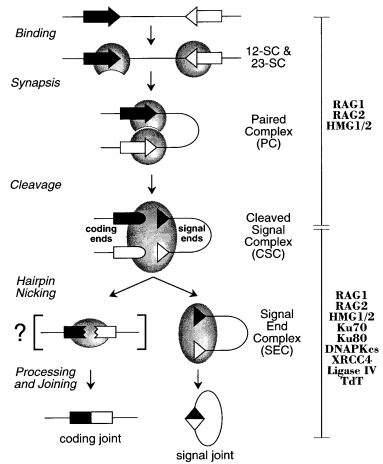
\includegraphics[width=1\linewidth]{VDJ_RAG_action}
%	\caption[Modelo das proteínas na linha germinal sujeita à recombinação VDJ.]{Modelo das proteínas sujeitas à recombinação V(D)J. Os triângulos representam as RSSs e os segmentos gênicos são os retângulos. \cite{introMain2}}
%	\label{fig:vdjragaction}
%\end{figure}

\begin{wrapfigure}{r}{0.4\linewidth}
	\centering
	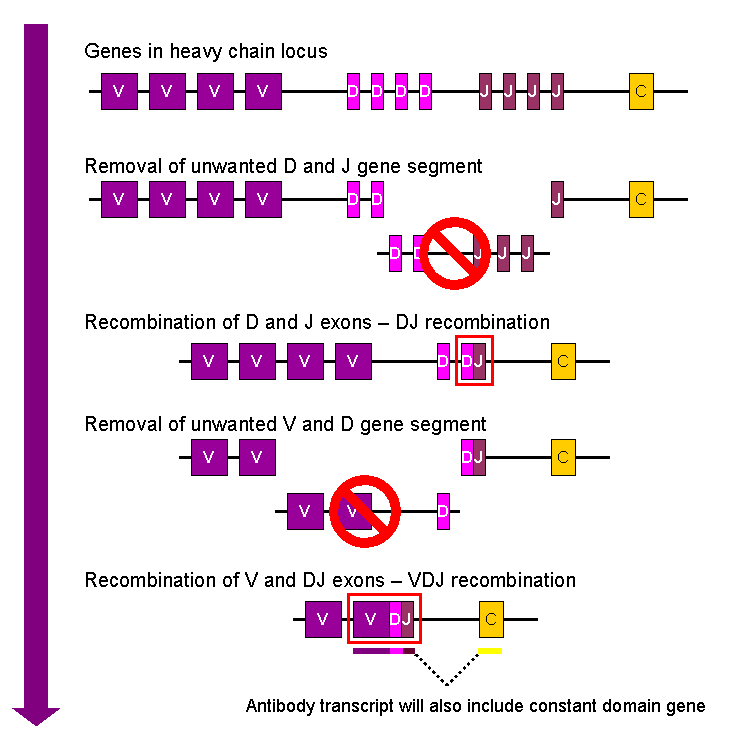
\includegraphics[width=1\linewidth]{VDJ_recombination}
	\caption[Esquema da recombinação V(D)J.]{Esquema da recombinação V(D)J \cite{fig:RAGscheme}.}
	\label{fig:vdjrecombination}
\end{wrapfigure}

A recombinação V(D)J requer ambos RAGs 1 e 2 (cujo conjunto é chamado de complexo RAG) para iniciar, sendo eles responsáveis pelo corte de seções de DNA que se encontram entre os segmentos gênicos (embora as funções específicas de cada RAG ainda não estejam esclarecidas). O complexo RAG vai se prender aos chamados RSSs (\textit{Recombination signal sequences}), os quais sinalizam quais partes dos segmentos serão utilizados para a composição do exon final \cite{main}. Cada RSS contém um heptâmero e um nonâmero conservados e um espaçamento entre eles. A sinalização promovida pelos RSSs se dá, também, pelo comprimento dos espaçamentos: em geral, os complexos RAG só atuam em pares de RSSs com espaçamentos distintos, especificamente entre os 12-RSS e 23-RSS (conhecida como ``regra 12/23'', o que se dá por conta da eficiência dessa reação), onde o número indica a quantidade de pares de base no espaçamento da sequência.

A figura \ref{fig:vdjrecombination} ilustra as etapas descritas do processo de recombinação V(D)J em linhas gerais%
\footnote{A descrição completa da ação das proteínas RAG está além do escopo desse trabalho, mas a descrição dada justifica sua indispensabilidade para o processo de recombinação.}.

A motivação do estudo das RAGs e das RSSs é a compreensão desse mecanismo biológico que é essencial para o sistema imunológico adaptativo presente em diversos animais, incluindo os seres humanos.

\chapter{Metodologia}

\section{Motivação da metodologia utilizada}

Alguns pesquisadores anteriores à \citeonline{main,flRAGpur1,flRAGpur2,flRAGpur3,flRAGpur4} fizeram uso de métodos simplificados que aproveitaram a alta solubilidade da parte central das RAGs (\textit{core RAG-1/2}) para estudar seu comportamento \textit{in vitro}. Neste trabalho, no entanto, descreverei a metodologia utilizada para a purificação das RAGs em sua total extensão (\textit{full-length RAG-1/2}) --- especificamente, o método por \citeonline{main}, que foi o artigo mais completo que encontrei sobre o tópico. O método é mais complexo porém é necessário para o estudo efetivo dessas proteínas, como fora reconhecido por \citeonline{coreXflRAG1,coreXflRAG2,coreXflRAG3,coreXflRAG4}. De acordo com esses pesquisadores, as partes ``não-centrais'' das RAGs ajudam a regular a atividade do complexo \textit{in vivo}, e por isso é essencial purificar as proteínas completas a fim de entender melhor seu comportamento.

\section{Vetores de expressão}

Para a produção de RAGs para esse estudo, os pesquisadores utilizaram um processo de múltiplas etapas para a geração de vetores de expressão apropriados:
\begin{enumerate}[label=\roman*.]
	\item Primeiramente, temos o uso de baculovírus como vetores de expressão, os quais foram utilizados para conseguir as partes centrais das RAGs (fundidas à proteínas ligantes de maltose).
	\item Depois, temos a subclonagem dos fragmentos de DNA dessas proteínas para o pcDNA1 como vetor de expressão mamífero.
	\item Utilizando o DNA complementar preparado no laboratório de S. Desiderio, os pesquisadores conseguiram gerar as porções com as partes não centrais das RAGs.
	\item Então, há a produção de diversas variantes mutantes das RAG-1/2 por PCR.
	\item Várias formas das RAGs foram inteiramente subclonadas em pcDNA1 e propagadas em estirpes de \textit{Escherichia coli}.
	\item Por fim, os plasmídeos foram purificados das colonias de bactérias.
\end{enumerate}

\section{Expressão das proteínas}

Ainda seguindo a metodologia de \citeonline{main}, na etapa de expressão, os pesquisadores utilizaram culturas celulares de células HEK (\textit{Human Embryonic Kidney}) 293 para expressar as proteínas RAG transientemente, a fim de purificá-las depois.

As células foram mantidas sob condições normais úmidas (\SI{37}{\degreeCelsius} e 5\% \ce{CO2} --- condições corporais) em um DMEM (\textit{Dulbecco's modified Eagle medium} --- meio de cultura artificial utilizado para manter as células de uma cultura), especificamente uma variante com alta glicose, L-glutamina e cloridrato de piridoxina (Invitrogen Life Technologies) suplementado com 50 unidades/\si{\milli\liter} de penicilina G e estreptomicina à \SI{50}{\micro\gram\per\milli\liter} (BioWhittaker, Walkersville, MD) e 10\% (v/v) de soro fetal bovino (FBS) (HyClone, Logan, UT)\footnote{Os pesquisadores também usaram FBS de outras marcas, com resultados semelhantes.}.

O meio de cultura final foi filtrado esterilmente por uma membrana de acetato de celulose de \SI{0.45}{\milli\meter} antes do uso (sistema de filtro de \SI{500}{\milli\liter} da Corning). As células cresceram à confluência em placas de petri de \SI{10}{\centi\meter}, foram resuspensas no mesmo meio e passadas para um meio fresco (diluídas em proporção 1:5) no dia anterior à transfecção.

Na manhã seguinte, aspiraram o meio e trocaram-no por \SI{10}{\milli\liter} de um novo meio, retornando à incubadora por \SI{3}{\hour}. Para transfecção transiente (onde não há integração do genoma externo), os pesquisadores recorreram ao procedimento de transfecção utilizando a PEI (\textit{polyethylenimine} --- Polysciences Inc., Warrington PA), que é o veículo para entrada na célula eucarionte. Eles prepararam uma solução aquosa padrão de PEI (\SI{1}{\micro\gram\per\milli\liter} levada ao pH \num{7.0} por adição de \ce{HCl}) e guardada em frações à \SI{-80}{\degreeCelsius}. A solução padrão foi preparada imediatamente após a abertura de uma nova garrafa de PEI.

O DNA do plasmídeo era adicionado ao \ce{NaCl} à uma concentração de \SI{0.9}{\percent} (m/v; filtrado esterilmente) numa concentração final de \SI{10}{\micro\gram\per\milli\liter}. Então adicionaram \SI{5}{\micro\gram} do vetor de expressão de cada RAG, para que houvesse co-expressão.

O PEI foi então adicionado até uma concentração final de \SI{30}{\micro\gram\per\milli\liter}. Após agitar as amostras por vórtice brevemente, elas foram incubadas por \SI{10}{\minute} à \SI{25}{\degreeCelsius} e então \SI{1}{\milli\liter} da mistura de DNA-PEI foi adicionada à cada prato de células HEK 293.

Para cada preparação de proteínas RAG, duas soluções de DNA-PEI foram montadas para transfecção de 14 placas de células 293. Após a incubação de \SI{48}{\hour}, o meio foi aspirado e sete pratos foram colhidos em \SI{5}{\milli\liter} de tampão estéril fosfato-salino (PBS) com EDTA (PBS-EDTA, \SI{137}{\milli\molar} \ce{NaCl}, \SI{27}{\milli\molar} \ce{KH2PO4}, \SI{14}{\milli\molar} \ce{Na2HPO4}, \SI{2}{\milli\molar} EDTA) por placa e coletados em um tubo cônico de \SI{50}{\milli\liter} sobre gelo. Os tubos foram centrifugados à $ 274g $ ($ g $ é a aceleração da gravidade) por \SI{10}{\minute} à \SI{4}{\degreeCelsius} (rotor Beckman GH3.8, \SI{1300}{\rpm}) e a sobrenadante foi aspirada. Aglomerados de células foram congelados em um banho de gelo/etanol e guardados à \SI{-80}{\degreeCelsius} até o uso.

\section{Purificação das proteínas}

Ambas MBP-RAG-1/2 coexpressas foram purificadas usando os mesmos procedimentos, todos feitos à \SI{4}{\degreeCelsius}:
\begin{enumerate}[label=\roman*.]
	\item Brevemente, cada aglomerado de células foi derretido sobre gelo e resuspenso em \SI{3.75}{\milli\liter} de um tampão A [\SI{10}{\milli\molar} de fosfato de sódio (pH \num{7.4}), \SI{0.5}{\molar} \ce{NaCl}, \SI{1}{\milli\molar} de ditiotreitol (DTT), \SI{0.25}{\percent} de polisorbato 20 (v/v)], carregado em um moedor de tecidos (Wheaton Science Produts, Millville, NJ), e sujeito à 20 movimentos de um macerador de tipo A.
	\item O lisado foi clarificado por centrifugação à $ \num{85000}g $ (rotor Beckman SW55Ti, \SI{30000}{\rpm}) por \SI{40}{\minute} à \SI{4}{\degreeCelsius} e os sobrenadantes coletados dos dois aglomerados foram passados por \SI{1}{\milli\liter} de resina de amilose (New England Biolabs, Ipswich, MA) e colocados em uma coluna de cromatografia Poly-Prep (\SI{9}{\centi\meter} de altura, cônico $ \num{0.8} \times \SI{4}{\centi\meter} $ de polipropileno --- Bio-Rad, Hercules, CA) equilibrada no tampão A pela gravidade.
	\item A coluna foi lavada com \SI{10}{\milli\liter} do tampão A contendo \SI{10}{\milli\molar} de maltose (os últimos \SI{5}{\milli\liter} sem o polisorbato 20) e as proteínas MBP‐RAGs foram eluídas com o tampão A contendo \SI{10}{\milli\molar} de maltose (também sem o polisorbato 20). As amostras contendo proteínas foram dialisadas (Spectra/Por \num{25000} MWCO, Spectrum Laboratories Inc., Rancho Dominguez, CA) contra um tampão R [\SI{25}{\milli\molar} Tris-\ce{HCl} (pH \num{8.0}, \SI{150}{\milli\molar} \ce{KCl}, \SI{2}{\milli\molar} DTT, e glicerol à 10\% (v/v))] por \SI{3}{\hour}.
	\item As frações foram ultracongeladas em nitrogênio líquido e guardadas à \SI{-80}{\degreeCelsius} até o uso.
	\item Brevemente, cada aglomerado de células derretido (dois no total) foi resuspenso em \SI{1.5}{\milli\liter} de um tampão de resuspensão (RSB) [\SI{10}{\milli\molar} Tris-\ce{HCl} (pH \num{7.4}), \SI{10}{\milli\molar} \ce{NaCl}, \SI{5}{\milli\molar} \ce{MgCl2}, \SI{1}{\milli\molar} fluoreto de fenilmetilsulfonil (PMSF), \SI{0.5}{\percent} IGEPAL CA-630 (NP-40; v/v)], e deixado inchar por \SI{5}{\minute}.
	\item Então, \SI{2.25}{\milli\liter} de tampão de amostras de Laemmli (LSB) frios [\SI{20}{\milli\molar} Tris–\ce{HCl} (pH \num{7.4}), \SI{1}{\molar} \ce{NaCl}, \SI{0.2}{\milli\molar} \ce{MgCl2}, \SI{1}{\milli\molar} PMSF, \SI{0.2}{\percent} IGEPAL CA‐630 (NP‐40; v/v)] foram adicionados e a amostra foi balançada à \SI{4}{\degreeCelsius} por \SI{1}{\hour}.
	\item O lisado então foi clarificado por centrifugação (como antes), e os sobrenadantes empoçados são aplicados à uma coluna preenchida com resina de amilose equilibrada em uma proporção de 1:\num{1.5} de tampões RSB:LSB (tampão RSB/LSB).
	\item A coluna é lavada com 5 volumes do tampão RSB/LSB e então com 4 volumes de \textit{Western Blot} (WB) [\SI{20}{\milli\molar} Tris–\ce{HCl} (pH \num{7.4}), \SI{0.5}{\molar} \ce{NaCl}, \SI{5}{\milli\molar} \ce{MgCl2}].
\end{enumerate}

\section{Ensaio de clivagem \textit{in vitro}}

Os autores de \citeonline{main} fizeram ensaios de clivagem utilizando um ensaio desenvolvido no laboratório Gellert \cite{refcleavage}. Nesse ensaio, há também partes com a proteína HMGB1 (\textit{High mobility group box 1}), que faz parte do estudo do artigo original.

\begin{quoting}[begintext={``},endtext={''\ (tradução livre)}]
	Em nosso laboratório, reações de clivagem são tipicamente montadas misturando $ \sim\SI{100}{\nano\gram} $ das proteínas RAG coexpressas (num total de \SI{4}{\micro\liter} de tampão de diálise [\SI{20}{\milli\molar} Tris–\ce (pH \num{8.0}), \SI{150}{\milli\molar} \ce{KCl}, glicerol à 10\%, \SI{2}{\milli\molar} DTT]) e substrato RSS ($ \sim\SI{0.02}{\pico\mol} $) em uma reação de \SI{10}{\micro\liter} contendo um tampão de amostra (ácido morfolinepropanosulfônico \SI{25}{\milli\molar} (MOPS)‐\ce{KOH} (pH \num{7.0}), \SI{60}{\milli\molar} glutamato de potássio, soro de albumina bovina \SI{100}{\micro\gram\per\milli\liter} e \SI{1}{\milli\molar} de \ce{MgCl2} ou \ce{MnCl2}). (...) As reações foram incubadas por \SI{1}{\hour} à \SI{37}{\degreeCelsius}, resfriadas adicionando 2 volumes de solução de carregamento de amostras (formamida à 95\%, \SI{10}{\milli\molar} de EDTA), e aquecidas à \SI{95}{\degreeCelsius} por \SI{2}{\minute}. Uma fração da amostra (\SI{5}{\micro\liter}) é fracionada em gel de sequenciamento de poliacrilamida à 15\% [19:1 acrilamida:metileno(bis)acrilamida] contendo ureia à \SI{7}{\molar}, e os produtos de clivagem são visualizados usando uma tela de fosforimagem (Storm 860; Molecular Dynamics‐GE Healthcare, Piscataway, NJ).
\end{quoting}

A figura \ref{fig:figura} foi retirada de \citeonline{main}. A legenda é uma tradução livre de trechos selecionados da legenda original.

\begin{figure}
	\centering
	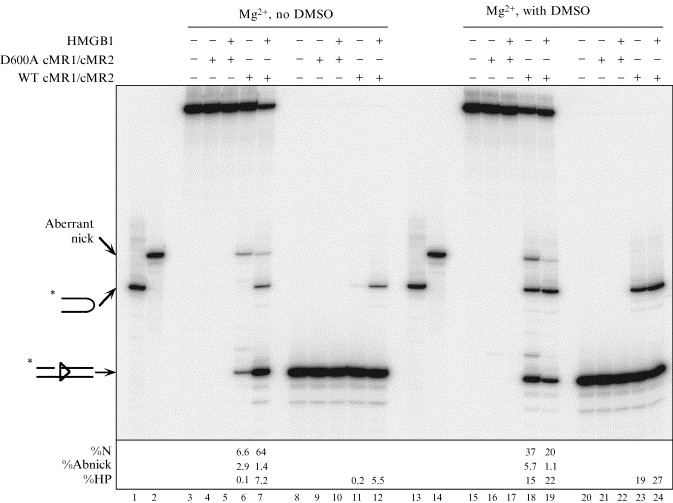
\includegraphics[width=0.7\linewidth]{figura}
	\caption[Ensaio de clivagem.]{Ensaio de clivagem \textit{in vitro} usando proteínas \textit{core} MBP-RAGs (MRs) purificadas e coexpressas e \textit{full-length} HMGB1 purificado. Substratos de 23-RSS intactos (faixas 3–7 e 15–19) ou ``nicked'' (faixas 8–12 e 20–24) foram incubados com um complexo RAG selvagem cataliticamente inativo (D600A cMR1/cMR2 ou sem cMR1/cMR2, respectivamente) em reações de clivagem padrão \textit{in vitro} contendo \ce{Mg2+} na ausência (faixas 3–12) ou na presença (faixas 15–24) de dimetilsulfóxido à 20\%, com ou sem HMGB1 adicionado (\SI{300}{\nano\gram}) como indicado acima do gel. \cite{main}}
	\label{fig:figura}
\end{figure}

%A figura \ref{fig:scheme} provém de outro artigo \cite{figuraabencoada}, porém usa o mesmo método de purificação que o artigo adotado na descrição metodológica presente nesse trabalho \cite{main}. Essa figura ilustra

%\begin{figure}
%	\centering
%	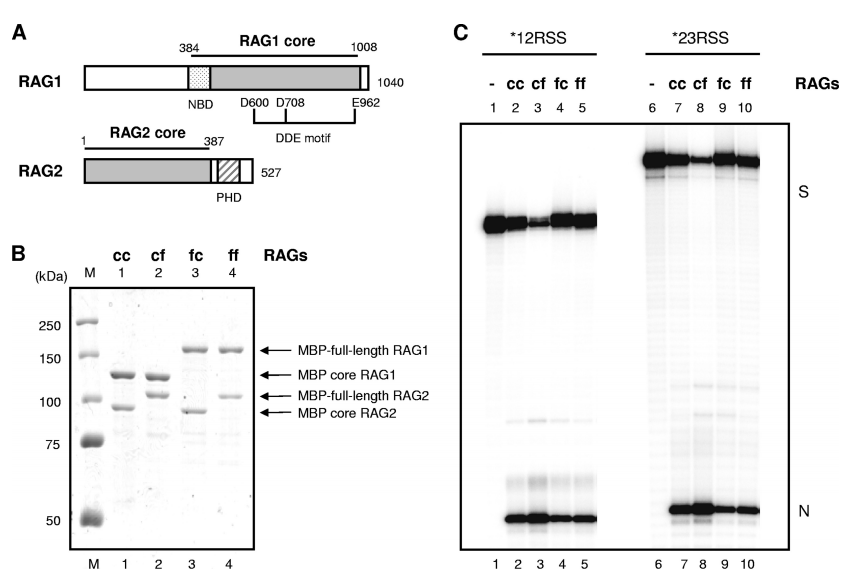
\includegraphics[width=0.7\linewidth]{scheme}
%	\caption[Esquema com testes realizados em RAGs]{As proteínas \textit{full-length} RAG estavam tão ativas quanto as \textit{core} RAG \textit{in vitro}. (A) Representação esquemática das RAG-1 e RAG-2. Núcleo da RAG-1, aa 384 até 1008; NBD, domínio nonâmero-ligante, aa 389 até 446; motivo DDE, aa 600, 708 e 962. Núcleo da RAG-2, aa 1 até 387; PHD finger, aa 414 até 481. (B) Proteínas RAG analisadas por SDS-PAGE. 1ª faixa, \textit{core} MBP-RAG-1/\textit{core} MBP-RAG-2 (cc); 2ª faixa, \textit{core} RAG-1/\textit{full-length} RAG-2 (cf); 3ª faixa, \textit{full-length} MBP-RAG-1/\textit{core} MBP-RAG-2 (fc); 4ª faixa, \textit{full-length} MBP-RAG-1/\textit{full-length} MBP-RAG-2 (ff). Cada combinação proteíca foi expressa em células 293T e purificado por cromatografia de resina de amilose. Proteínas purificadas foram fracionadas em SDS-PAGE com massas moleculares padrão e coradas com Coomassie blue. (C) Complexos de proteínas RAG purificados foram testados em ``nicking assays'' \textit{in vitro} com substrato de oligonucleotídeos 12-RSS (esquerda) ou 23-RSS (direita) por \SI{30}{\minute} à \SI{37}{\degreeCelsius}, como esboçado em ``Materials and Methods''. Os produtos foram analisados em géis de desnaturação à 10\%, seguidos de auto-radiografia. As posições de produtos de subtrato (S) e ``nicked'' (N) são indicados na margem direita. (tradução livre de \citeonline{figuraabencoada})}
%	\label{fig:scheme}
%\end{figure}


\chapter{Resultados}

\section{Introdução}

Utilizando dados do \url{uniprot.org}\footnote{
Dados retirados de \url{https://www.uniprot.org/uniprot/P15918} e \url{https://www.uniprot.org/uniprot/P55895}.}, temos que as massas das RAGs 1 e 2 são, respectivamente \SI{119097.05}{\dalton} e \SI{59241.02}{\dalton}. A RAG-1 possui 1043 aminoácidos em sua sequência, enquanto a RAG-2 possui 527. As proteínas são encontradas no núcleo celular, que possui um pH em torno de \num{7.3} \cite{phmes}.

\section{Sequências de aminoácidos}

Abaixo, seguem as sequências de aminoácidos das proteínas:

\subsection{RAG-1:}
\begin{texshade}{P15918.fasta}
	\noblockskip
	\residuesperline*{50}
	\hideconsensus
\end{texshade}

\subsection{RAG-2:}
\begin{texshade}{P55895.fasta}
	\noblockskip
	\residuesperline*{50}
	\hideconsensus
\end{texshade}

\section{pIs, cofatores e resíduos de aminoácidos notáveis}

As proteínas RAG-1 e RAG-2 possuem um pIs teóricos calculados de 8.94 e 5.55,\footnote{Dados retirados de \url{https://web.expasy.org/cgi-bin/protparam/protparam1?P15918@noft@} e \url{https://web.expasy.org/cgi-bin/protparam/protparam1?P55895@noft@}.} respectivamente. A proteína RAG-1 possui dois cofatores não-orgânicos, nomeadamente o \ce{Mg^2+} e o \ce{Mn^2+}, os quais são responsáveis pela função de clivagem do complexo RAG \cite{RAG1cof}.

Para a RAG-1, temos que os resíduos D600 (aspartato na posição 600), D708 e E962 (glutamato na posição 962) são os mais importantes, sendo que suas funções ainda não foram bem determinadas, porém muitas evidências indicam que os resíduos D600 e D708 são responsáveis pela coordenação de um íon divalente (cofator), função essencial à catálise da proteína. De forma análoga, o E962 possui uma função essencial para a catálise, porém não é relacionada à ligação iônica \cite{impRAG1}. Mais recentemente, há também estudos que mostram que os resíduos D546 e E547 são essenciais para a formação do complexo RAG \cite{newandcool}.

Temos a estrutura da RAG-1 com os resíduos interessantes marcados por \citeonline{newandcool} na figura \ref{fig:rag1struMarked}. Podemos notar que quase todos os resíduos (com exceção do D600) se encontram em alfa-hélices, em posições internas.

%De acordo com o site UniProt, 

%\begin{figure}
%	\centering
%	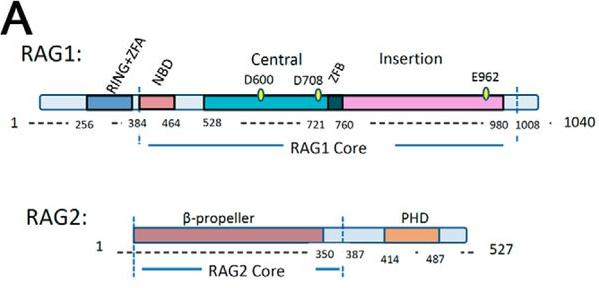
\includegraphics[width=0.7\linewidth]{RAGsstruschem}
%	\caption{Estrutura esquemática das RAGs. \cite{newandcool}}
%	\label{fig:RAGsstruschem}
%\end{figure}

%\begin{minipage}{0.49\linewidth}
	
	\begin{figure}
		\centering
		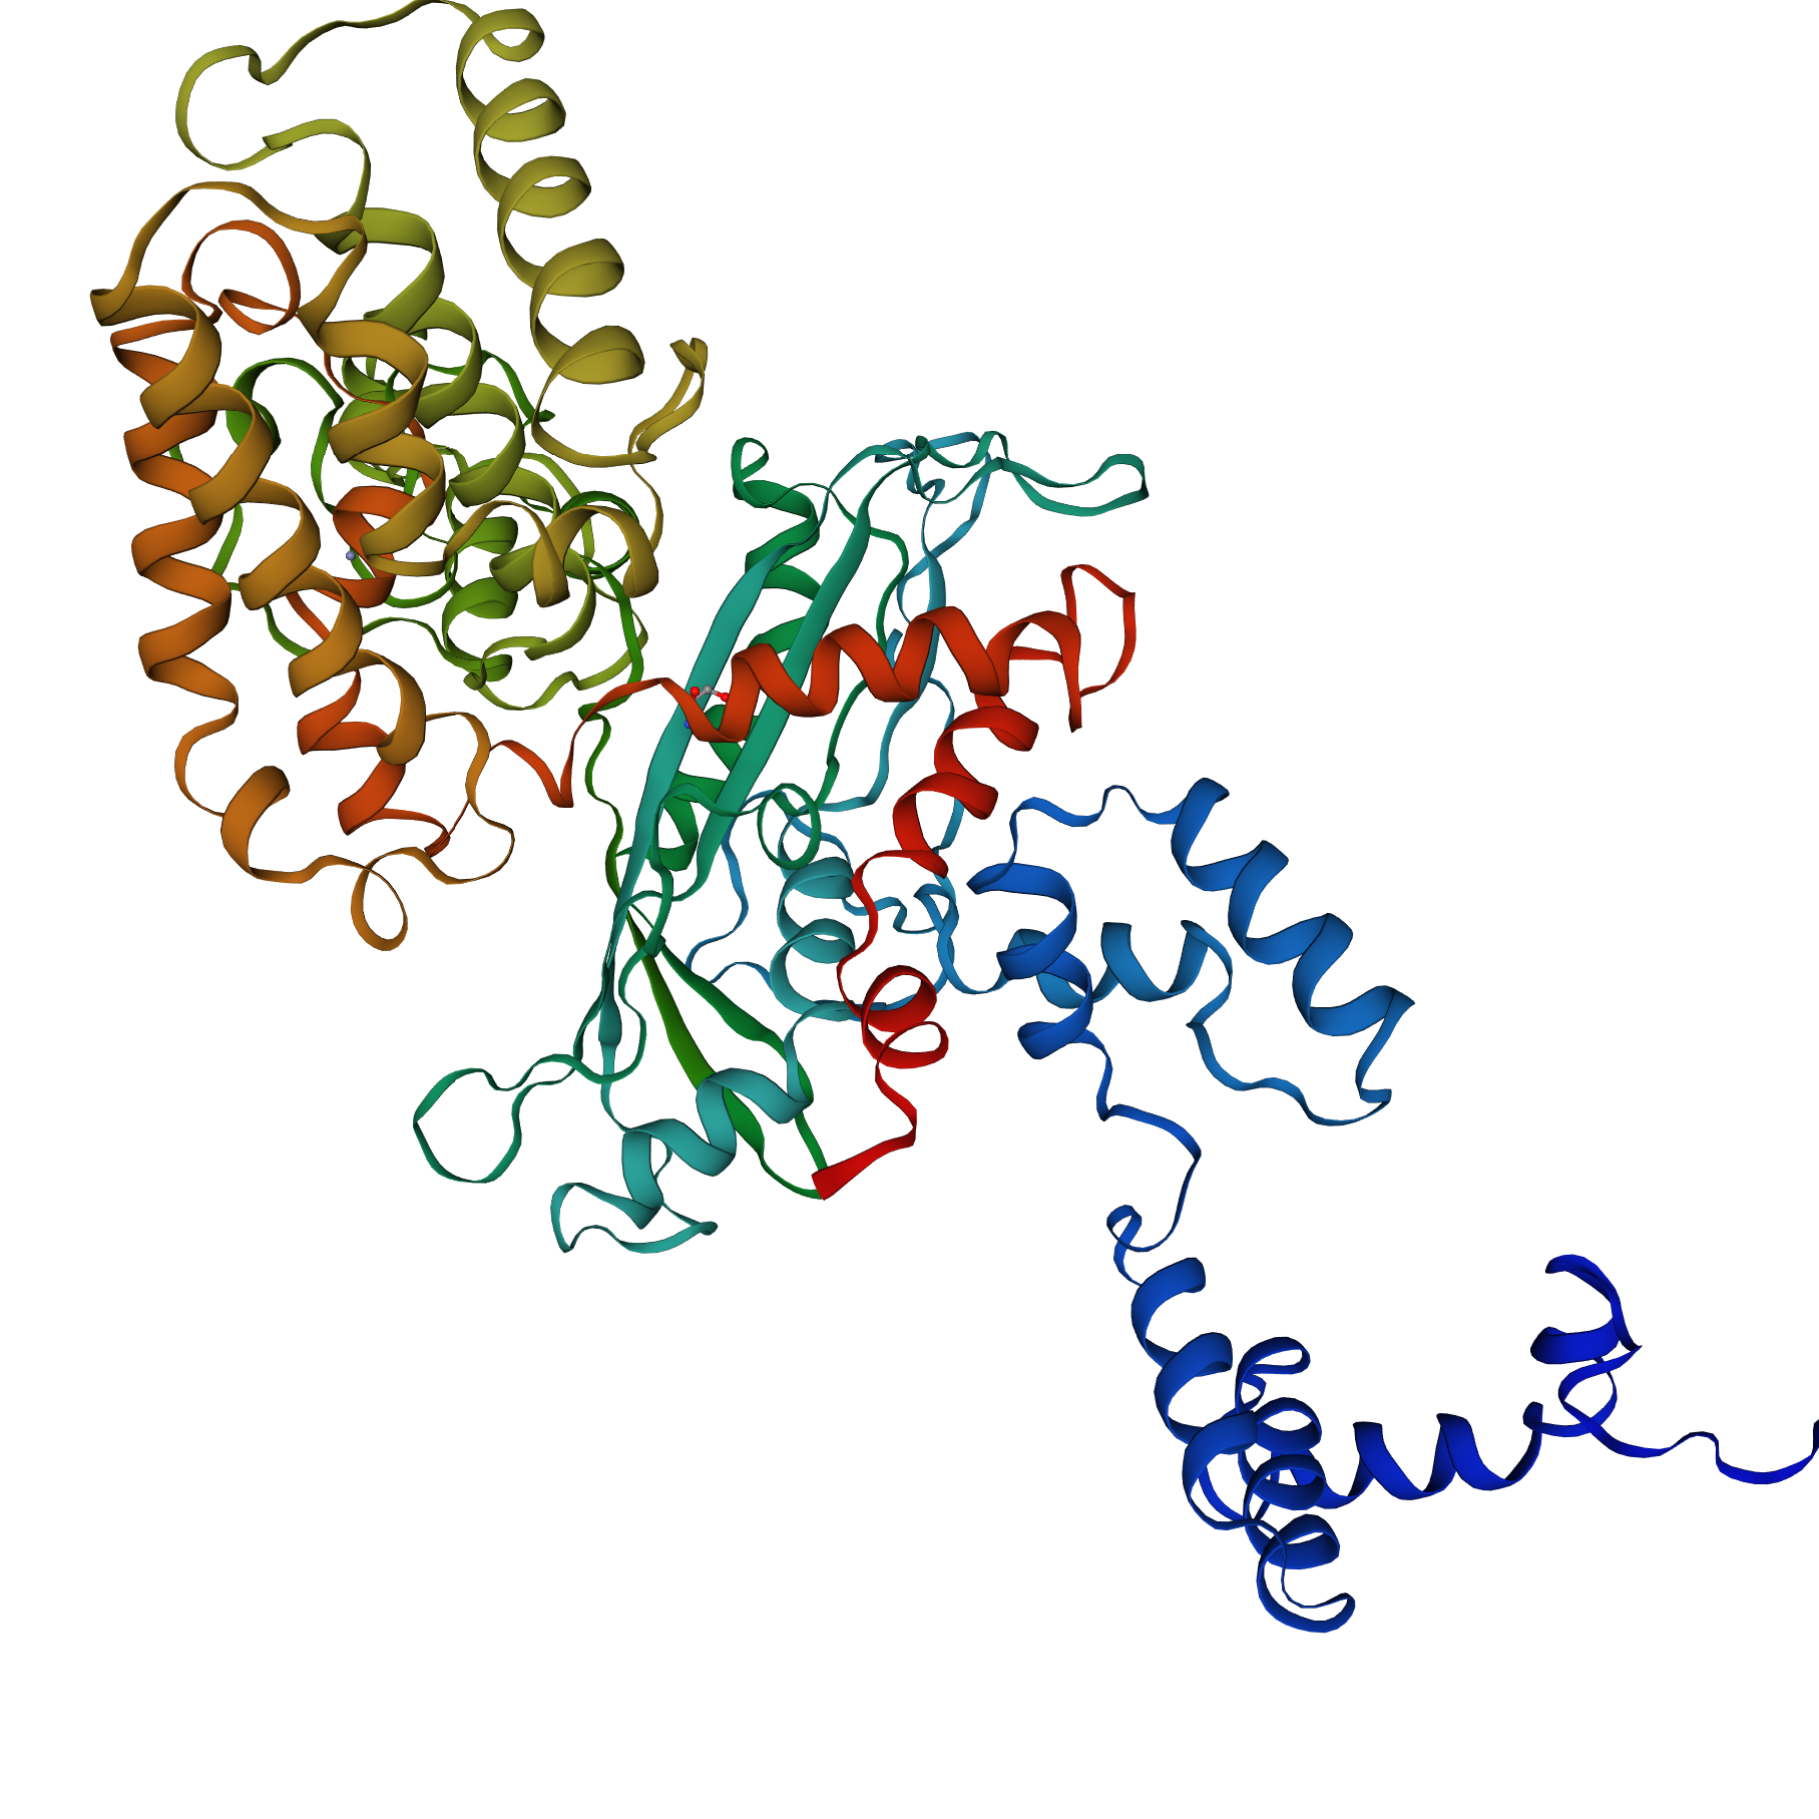
\includegraphics[width=0.5\linewidth]{RAG1stru}
		\caption[Estrutura da RAG-1.]{Estrutura da RAG-1. Retirada de \url{https://swissmodel.expasy.org/repository/uniprot/P15918?template=6oet.1.C&range=388-1010}}.
		\label{fig:rag1stru}
	\end{figure}

%\end{minipage}\hfill
%\begin{minipage}{0.49\linewidth}
	
	\begin{figure}
		\centering
		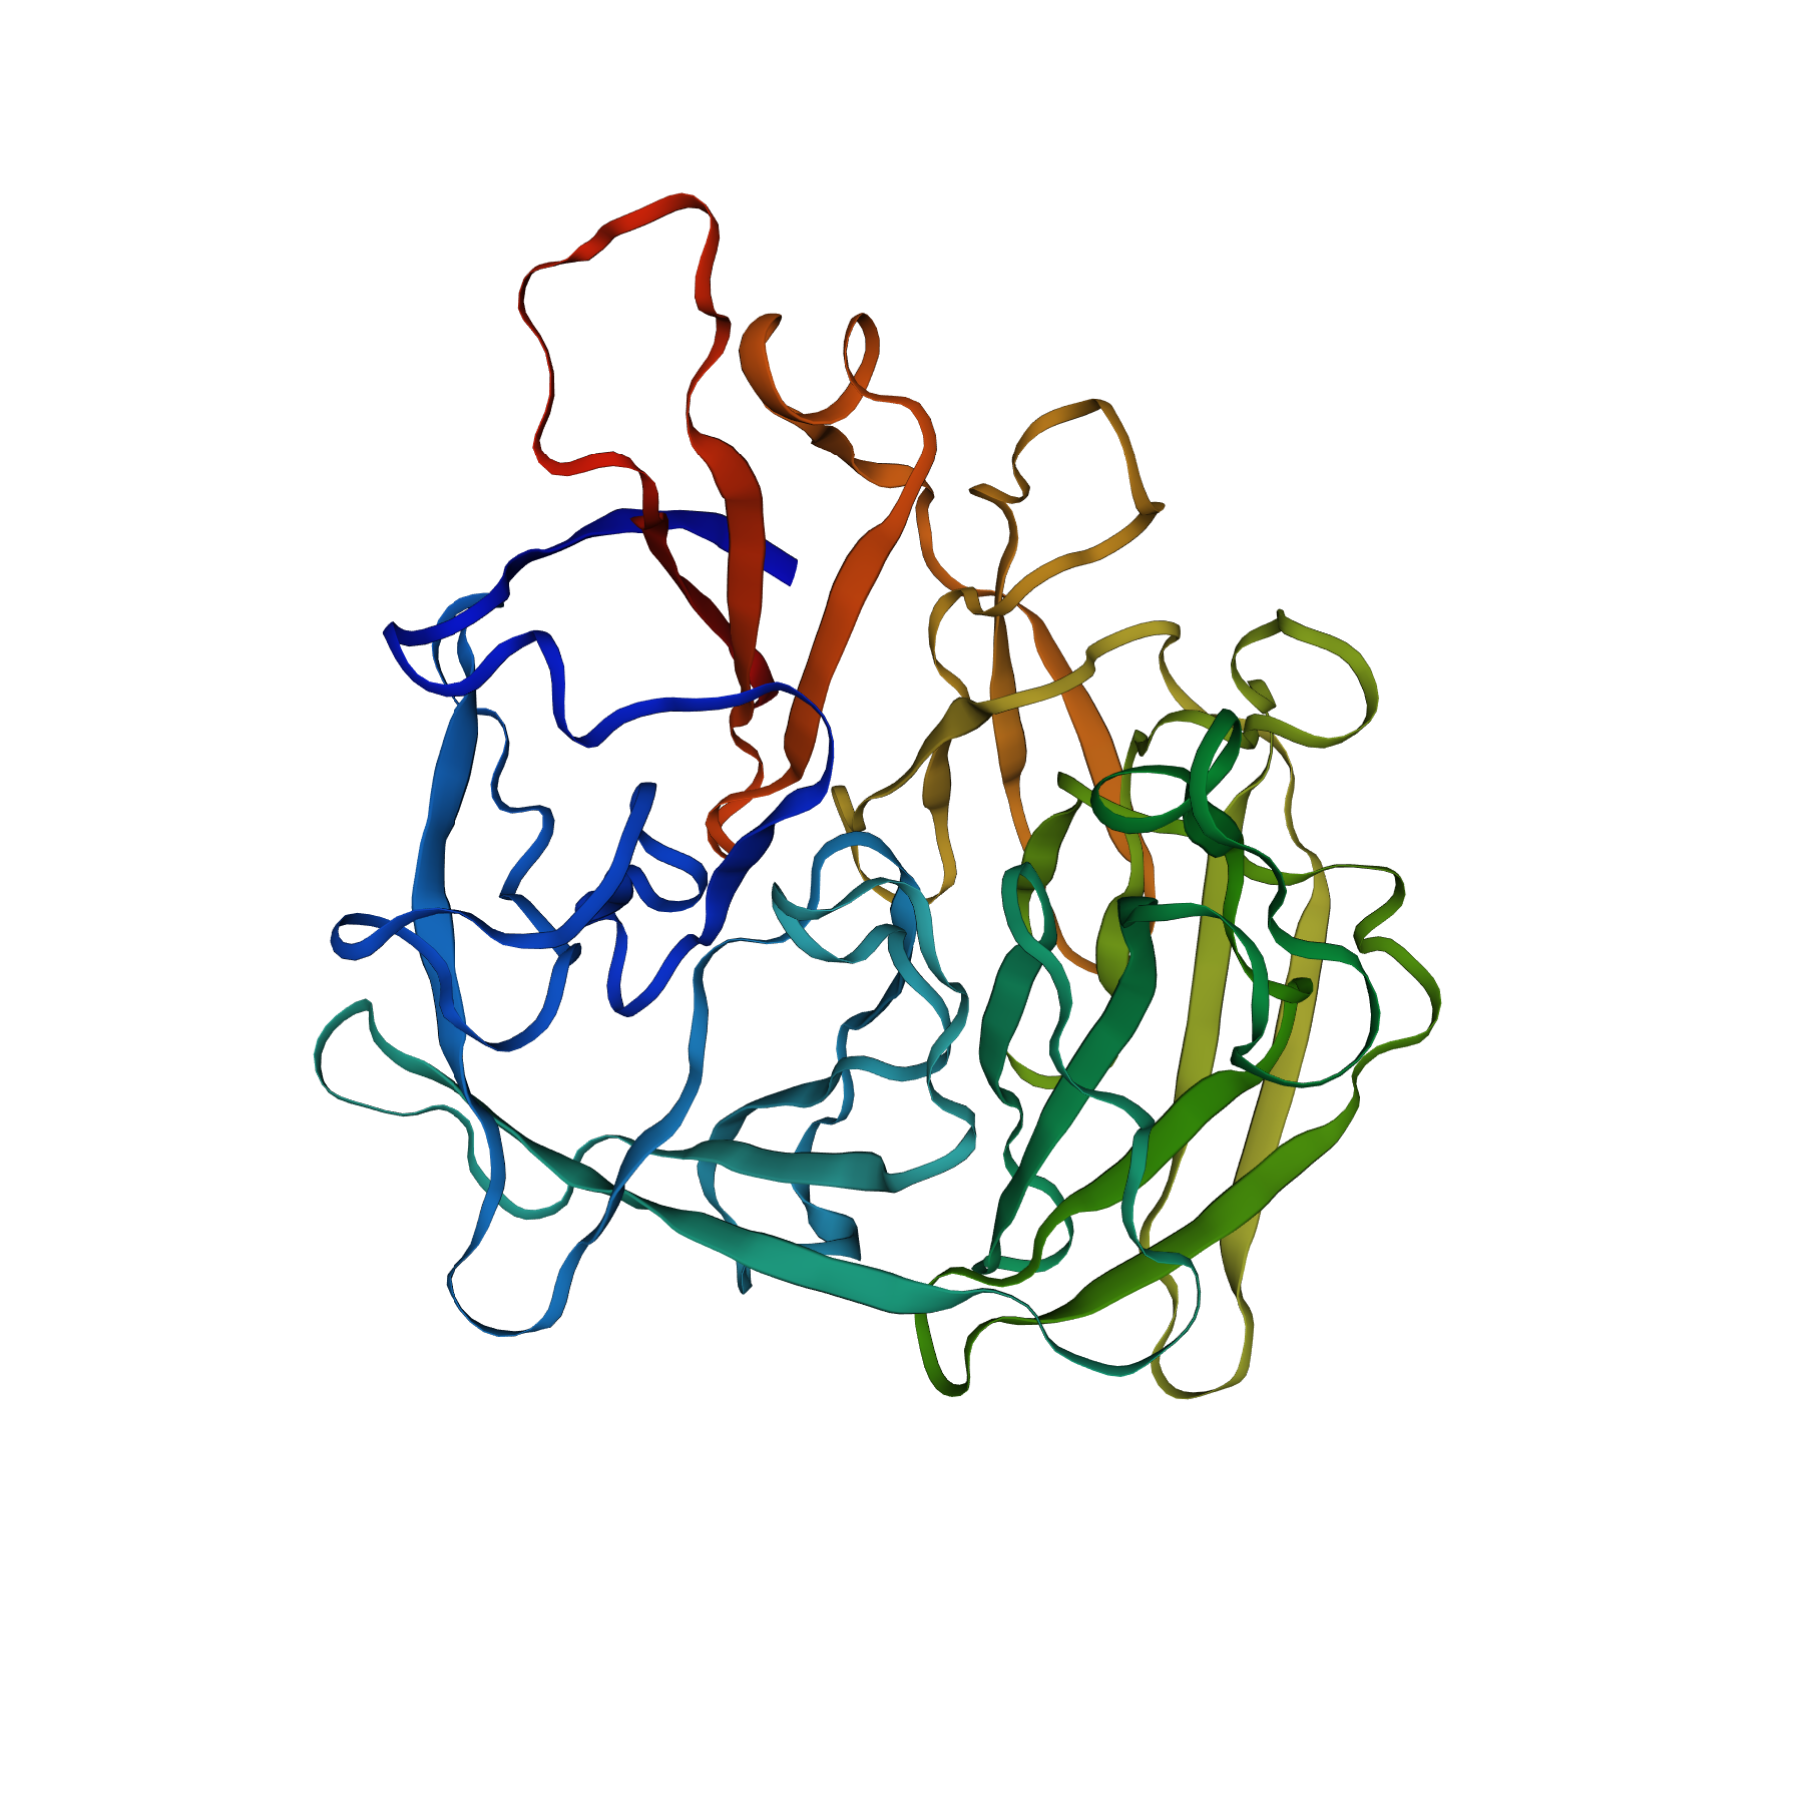
\includegraphics[width=0.5\linewidth]{RAG2stru}
		\caption[Estrutura da RAG-2.]{Estrutura da RAG-2. Retirada de \url{https://swissmodel.expasy.org/assess/5f57c7d8b6a2947dd7379540/01}}.
		\label{fig:rag2stru}
	\end{figure}

%\end{minipage}

\begin{figure}
	\centering
	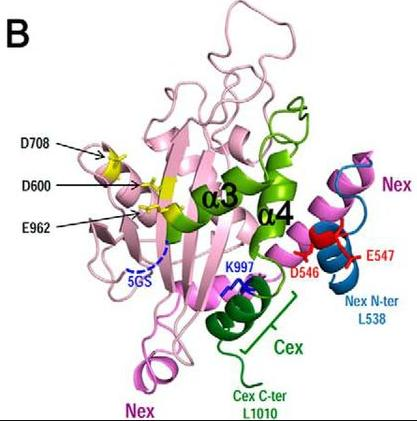
\includegraphics[width=0.5\linewidth]{RAG1stru2}
	\caption[Estrutura da RAG-1 com resíduos de aminoácidos marcados.]{Estrutura da RAG-1 com resíduos de aminoácidos marcados \cite{newandcool}.}
	\label{fig:rag1struMarked}
\end{figure}


\begin{figure}
	\centering
	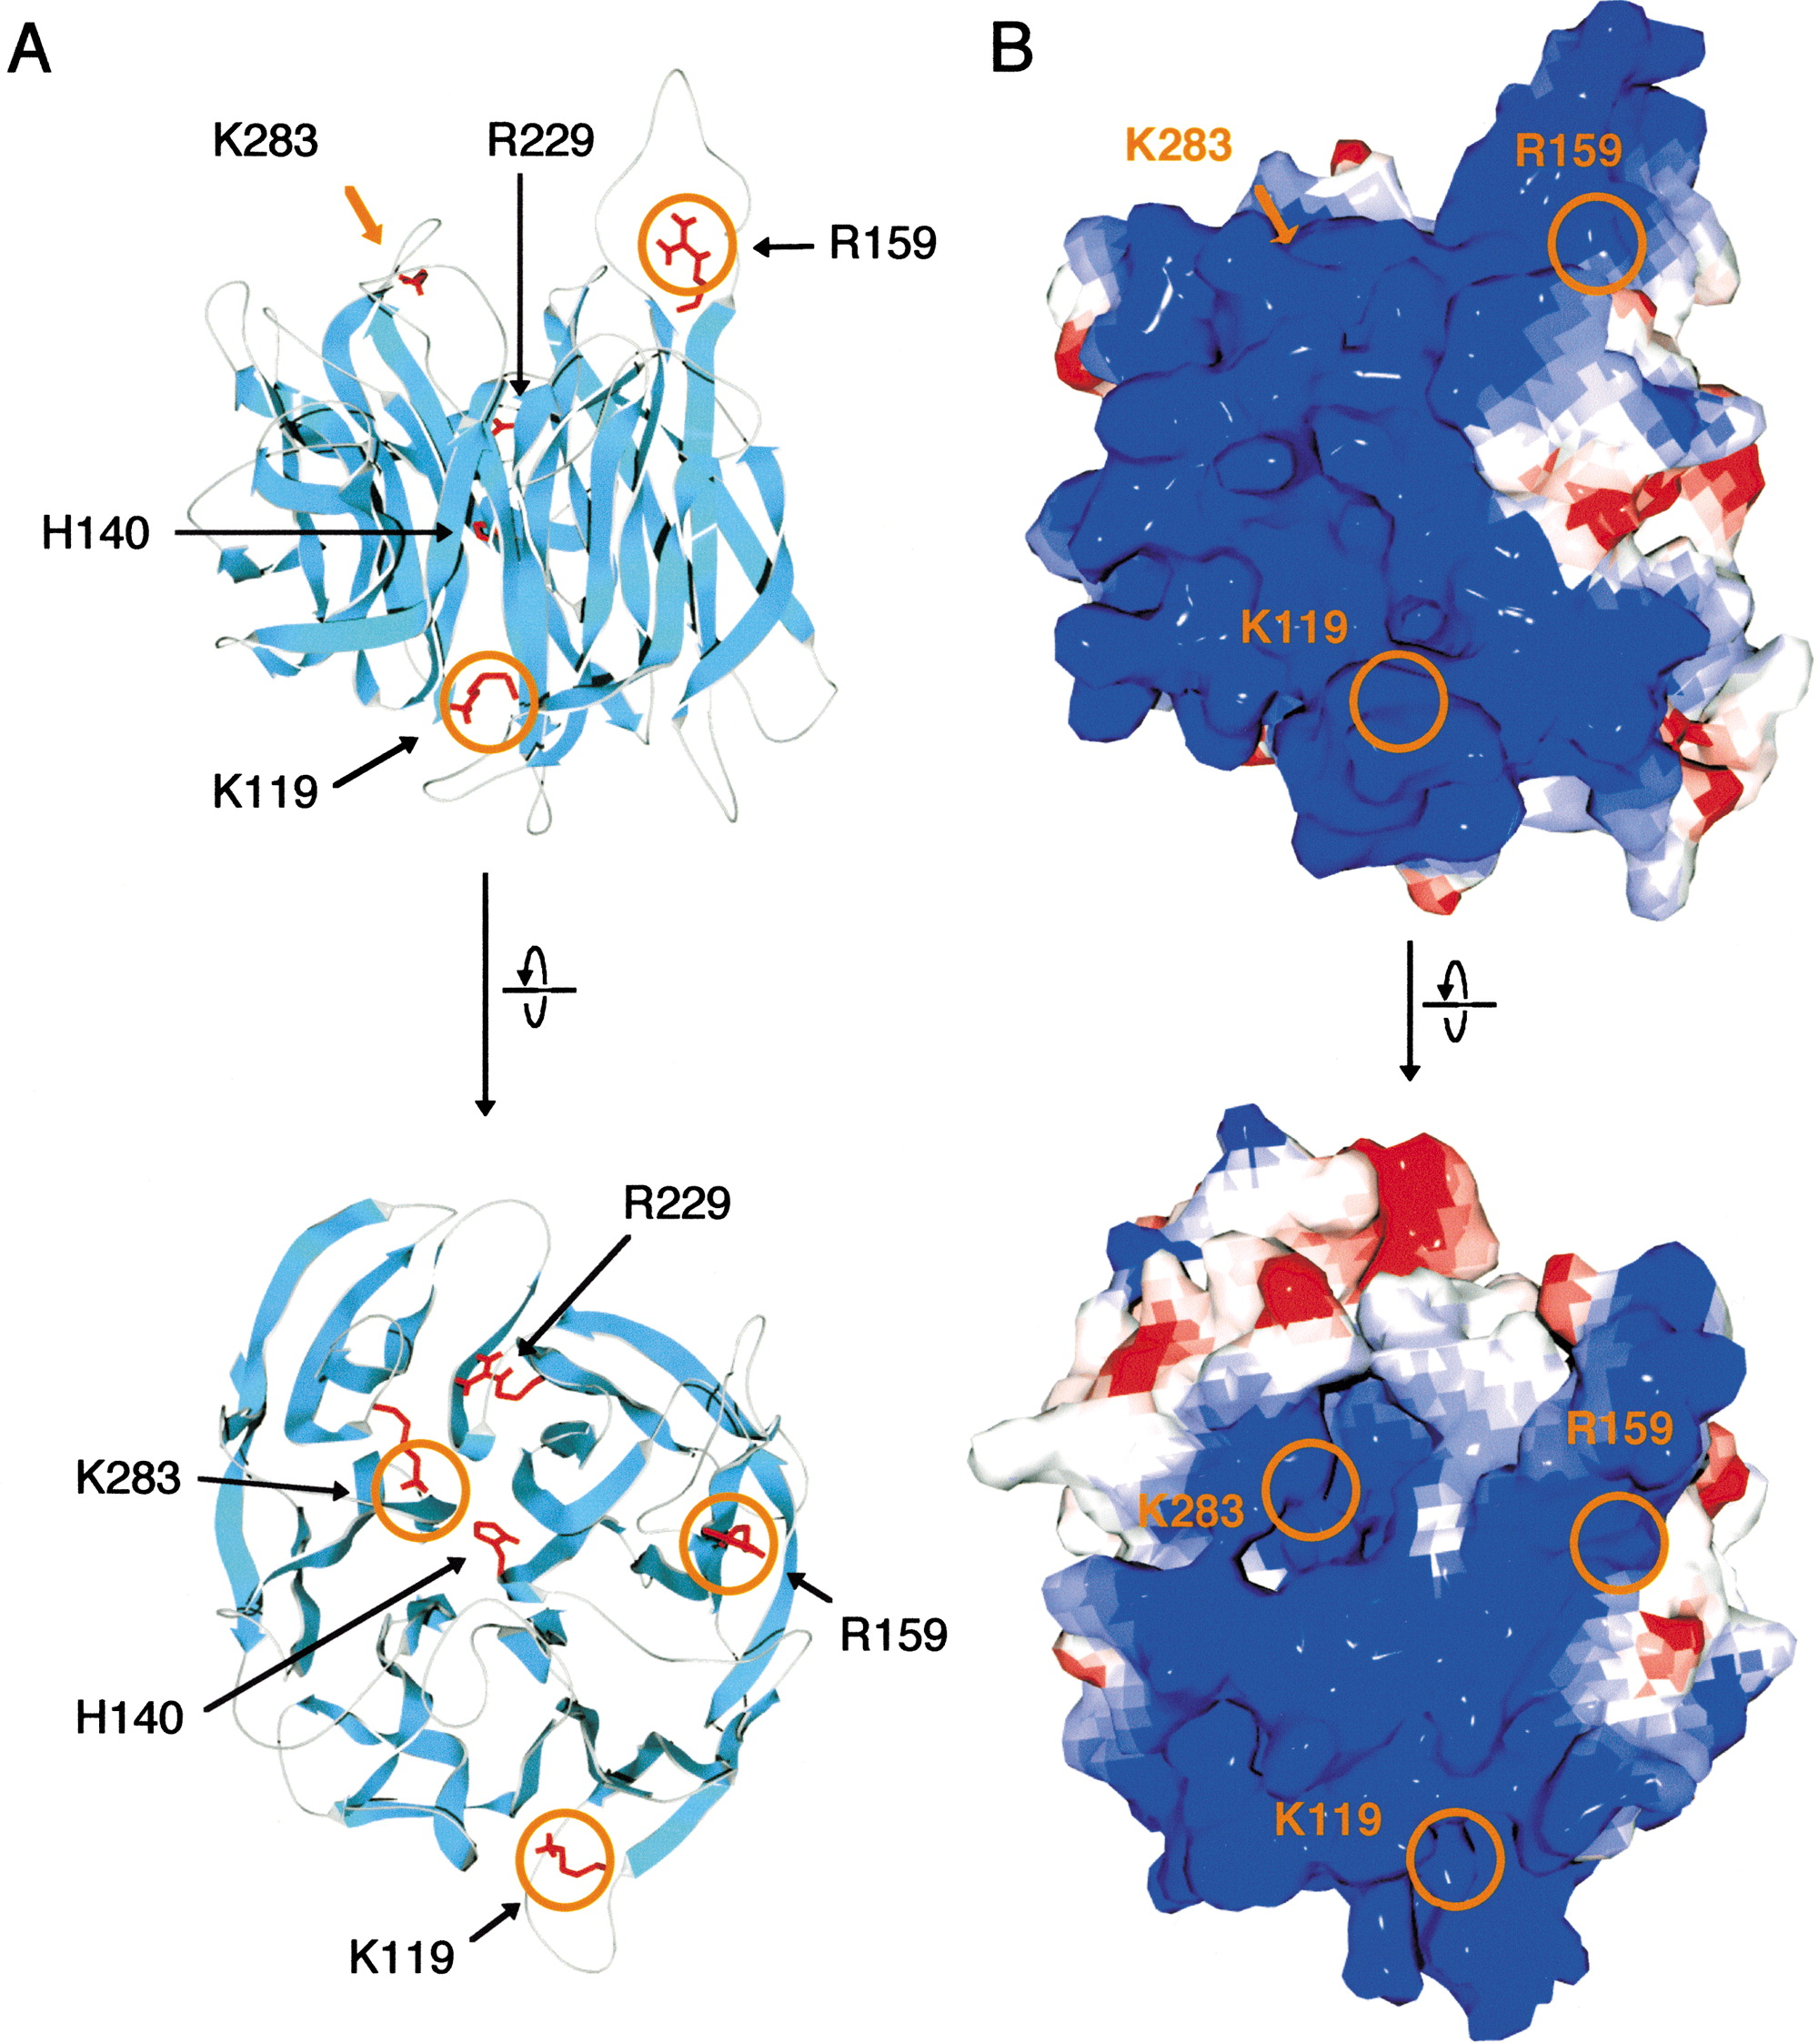
\includegraphics[width=0.7\linewidth]{RAG2struMarked}
	\caption[Estrutura da RAG-2 com resíduos de aminoácidos marcados, as linhas \texorpdfstring{$ \beta $}{beta} estão marcadas em azul.]{Estrutura da RAG-2 com resíduos de aminoácidos marcados, as linhas $ \beta $ estão marcadas em azul \cite{newandcool}.}
	\label{fig:rag2struMarked}
\end{figure}

%In summary, the results from the one-hybrid system demonstrate that the basic residues at positions 119, 140, 159, 229, and 283 within RAG2 are critical for RAG1-RAG2-DNA complex formation in vivo.

Já na RAG-2, \citeonline{impRAG2} determinaram que os resíduos K119 (lisina na posição 119), H140 (histidina na posição 140), R159 (arginina na posição 159), R229 e K283 eram essenciais para a formação do complexo RAG \textit{in vivo}, e os resíduos R73, K119, R137, H140, R159, R229 e K283 são essenciais para a catálise do complexo, e também para a formação de um complexo enzima-subtrato estável, assim como os resíduos S104 (serina na posição 104) e Y108 (tirosina na posição 108). Esses últimos, porém, afetaram a catálise em menor escala.

Temos a estrutura da RAG-2 com os resíduos interessantes marcados por \citeonline{newandcool} na figura \ref{fig:rag2struMarked}. Pela figura, é visível que os resíduos K119, R159 e K283 estão na superfície da proteína, enquanto os outros são encontrados internamente.

\section{Características das cadeias laterais dos resíduos importantes das RAGs}

Abaixo seguem algumas características importantes das cadeias laterais dos resíduos mencionados na subseção anterior:

\begin{itemize}
	\item[Arginina:] Básica e apolar, hidrofílica em pHs básico e neutro.
	\item[Aspartato:] Ácida e apolar, hidrofílica em pHs básico e neutro.
	\item[Glutamina:] Ácida e apolar, neutra em pH básico e hidrofílica em pH neutro.
	\item[Histidina:] Básica e apolar, Neutra em pH básico e hidrofílica em pH neutro.
	\item[Lisina:] Básica e apolar, hidrofílica em pHs básico e neutro.
\end{itemize}

\section{Mudanças conformacionais conhecidas}

Sabe-se que a trimetilação da histona H3 na lisina 4 (H3K4me3) produz uma mudança conformacional relacionada à atividade do complexo RAG (especificamente à atividade regulatória da RAG-2 --- regulação alostérica) \cite{putariarandom}.

\chapter{Conclusões}

Durante a realização desse trabalho compreendi melhor as conexões entre as diferentes partes de um estudo, e como se dá a exploração de uma proteína (expressão, purificação, produção de imagens, etc.).

Acredito que o aspecto mais interessante da minha exploração foi o estudo dos resíduos de aminoácidos. Os artigos desse tópico mostram como a estrutura da proteína afeta sua função na escala de uma única mutação, o que indica a robustez e a fragilidade (paradoxal) dos sistemas biológicos.

Também acho muito interessante a formação de vetores de expressão, pois há diversas formas de expressar uma mesma proteína por métodos que se assemelham a um ``LEGO de DNA''.

Sobre as RAGs, fiquei fascinada desde o princípio, pois o mecanismo de produção de linfócitos é tomado como garantido no dia-a-dia, mas é bastante complexo e detalhado (além de ser muito eficiente), e num momento de pandemia conseguimos apreciar o valor de um sistema imunológico funcional. Mesmo assim, conhecemos o mecanismo a mais de três décadas (Nobel de 1987), e ele ainda tem aspectos mal compreendido (função específica das RAGs).

\postextual

%\nocite{*}
\bibliography{bioP1}

% ----------------------------------------------------------
% Glossário
% ----------------------------------------------------------
%
% Consulte o manual da classe abntex2 para orientações sobre o glossário.
%
%\glossary

% ----------------------------------------------------------
% Apêndices
% ----------------------------------------------------------

% ---
% Inicia os apêndices
% ---
%\begin{apendicesenv}
%
%% Imprime uma página indicando o início dos apêndices
%\partapendices
%
%% ----------------------------------------------------------
%\chapter{Quisque libero justo}
%% ----------------------------------------------------------
%
%\lipsum[50]
%
%% ----------------------------------------------------------
%\chapter{Nullam elementum urna vel imperdiet sodales elit ipsum pharetra ligula
%ac pretium ante justo a nulla curabitur tristique arcu eu metus}
%% ----------------------------------------------------------
%\lipsum[55-57]
%
%\end{apendicesenv}
% ---


% ----------------------------------------------------------
% Anexos
% ----------------------------------------------------------

% ---
% Inicia os anexos
% ---
%\begin{anexosenv}
%
%% Imprime uma página indicando o início dos anexos
%\partanexos
%
%% ---
%\chapter{Morbi ultrices rutrum lorem.}
%% ---
%\lipsum[30]
%
%% ---
%\chapter{Cras non urna sed feugiat cum sociis natoque penatibus et magnis dis
%parturient montes nascetur ridiculus mus}
%% ---
%
%\lipsum[31]
%
%% ---
%\chapter{Fusce facilisis lacinia dui}
%% ---
%
%\lipsum[32]
%
%\end{anexosenv}

%---------------------------------------------------------------------
% INDICE REMISSIVO
%---------------------------------------------------------------------
%\phantompart
%\printindex
%---------------------------------------------------------------------

\end{document}
